\documentclass[conference]{IEEEtran}
\IEEEoverridecommandlockouts
\usepackage{cite}
\usepackage{amsmath,amssymb,amsfonts}
\usepackage{algorithmic}
\usepackage{graphicx}
\usepackage{textcomp}
\usepackage{xcolor}
\graphicspath{{figures/}{../../research/figures/}}
% IEEE-compliant float placement parameters (prevent float accumulation)
\renewcommand{\topfraction}{0.90}
\renewcommand{\bottomfraction}{0.85}
\renewcommand{\textfraction}{0.10}
\renewcommand{\floatpagefraction}{0.80}
\renewcommand{\dbltopfraction}{0.90}
\renewcommand{\dblfloatpagefraction}{0.80}
\setcounter{topnumber}{3}
\setcounter{bottomnumber}{3}
\setcounter{totalnumber}{5}
\setcounter{dbltopnumber}{2}
\def\BibTeX{{\rm B\kern-.05em{\sc i\kern-.025em b}\kern-.08em
    T\kern-.1667em\lower.7ex\hbox{E}\kern-.125emX}}

\begin{document}

\title{AN AI-POWERED SYSTEM FOR CORRELATING PHYSICAL ACTIVITY AND SUBJECTIVE MENTAL WELL-BEING\\
{\footnotesize Multimodal N-of-1 Mood Prediction with Wearable and NLP Fusion}
\thanks{Project Work, School of Computer Science and Engineering, VIT Chennai.}
}

\author{
\IEEEauthorblockN{Harsh Pratap Singh}
\IEEEauthorblockA{
  \textit{School of Computer Science and Engineering}\\
  \textit{Vellore Institute of Technology}\\
  Chennai, India\\
  harsh.devmail@gmail.com
}
\and
\IEEEauthorblockN{Dr. Saranya G}
\IEEEauthorblockA{
  \textit{School of Computer Science and Engineering}\\
  \textit{Vellore Institute of Technology}\\
  Chennai, India\\
  saranya@vit.ac.in
}
}

\maketitle

\begin{abstract}
Mental health affects nearly a billion people worldwide, yet the tools we use to assess it---periodic questionnaires and clinical interviews---are retrospective, rely on self-reporting, and use broad categories that miss day-to-day fluctuations. Wearable devices now offer a way to passively track physiological signals, but these signals alone cannot tell us \textit{why} someone feels the way they do. This paper presents MindfulMomentum, an end-to-end system that combines wearable data with natural language processing (NLP) on free-text journal entries to predict daily mood. We frame mood as a three-class problem (Low, Neutral, High) and train a separate, personalized model for each user rather than building one model for everyone. Using the PMData dataset (16 participants, multiple weeks of Fitbit data and daily wellness surveys), we engineer 22+ time-lagged features and compare six classifier families---Random Forest, XGBoost, LightGBM, Logistic Regression, SVM, and KNN---with Optuna hyperparameter tuning and TimeSeriesSplit cross-validation. The NLP pipeline uses RoBERTa for emotion scoring and Sentence-BERT for semantic theme detection. To evaluate the potential of NLP fusion, we conducted an ablation study using simulated emotion features correlated with ground-truth mood labels, since PMData does not include free-text journal entries. This ablation showed that adding emotion features improved mean macro-F1 from 0.674 to 0.793 (+0.119), a gain confirmed as statistically significant by a Wilcoxon signed-rank test ($p = 0.0077$). While these results use simulated proxies and will need validation with real journal data from the deployed app, they support our hypothesis that combining text-derived features with wearable data can meaningfully improve personalized mood prediction.
\end{abstract}

\begin{IEEEkeywords}
digital phenotyping, mood prediction, N-of-1 models, natural language processing, RoBERTa, wearable fusion, affective computing, ecological momentary assessment
\end{IEEEkeywords}

% ================================================================
% SECTION I: INTRODUCTION
% ================================================================
\section{Introduction}

\subsection{Background and Motivation}

Monitoring mental health in everyday life is hard. The standard tools---questionnaires like PHQ-9 for depression or the Perceived Stress Scale---are filled out every few weeks and depend on people remembering how they felt. They work well enough in clinical settings, but they suffer from recall bias and cannot capture the rapid ups and downs of daily mood~\cite{shiffman2008}.

Consumer wearables like Fitbit and Apple Watch have opened up a different approach. These devices continuously record step counts, heart rate, sleep patterns, and calories burned without requiring any effort from the user. Research in digital phenotyping has shown that these passive signals do relate to mood: fewer steps correlate with depressive episodes~\cite{saeb2015}, poor sleep predicts anxiety~\cite{gruber2011}, and higher resting heart rate is linked to stress~\cite{kim2018}. But here is the problem---physiological signals are inherently ambiguous. A day with zero steps could mean depression, or it could mean a lazy Sunday. The sensor tells you \textit{what} happened in the body, not \textit{why}.

This is where daily journaling comes in. When someone writes about their day, they naturally encode emotional context, situational details, and causal reasoning that no sensor can capture. With recent advances in transformer-based NLP, it has become practical to extract structured emotional signals from this kind of free text. Models like RoBERTa~\cite{liu2019roberta} and Sentence-BERT~\cite{reimers2019sbert} handle sarcasm, negation, and informal language far better than older lexicon-based tools like VADER~\cite{hutto2014vader}.

Despite having both data streams available, most work in computational mental health still uses only one modality at a time. Studies that do combine physiological and text data typically train a single population-level model across all users, which assumes that the relationship between sensor data and mood is the same for everyone~\cite{sano2018}. That assumption is clearly wrong. For some people, sleep quality drives their mood. For others, it is physical activity or social interaction~\cite{molenaar2009}. A one-size-fits-all model will inevitably fail for most individuals.

\subsection{The N-of-1 Personalization Paradigm}

The N-of-1 trial design, originally from clinical pharmacology~\cite{lillie2011}, addresses this by treating each person as their own experiment. In machine learning terms, this means training a separate model for each user using only their own data. The model learns that specific user's patterns---what affects \textit{their} mood---rather than learning a group average.

This approach has seen some adoption in mobile health research~\cite{suhara2017deepmood}, but existing systems rarely combine wearable features with text-derived features, and even fewer use modern transformer models for the NLP component. MindfulMomentum is designed to fill this gap.

\subsection{Research Contributions}

This paper makes four specific contributions:
\begin{enumerate}
    \item \textbf{Multimodal Feature Fusion:} We build a feature space that combines Fitbit physiological metrics, daily wellness self-reports, and NLP-derived emotion and theme features from journal text.
    \item \textbf{N-of-1 Evaluation:} We train and evaluate six classifier families independently for each of 16 participants, using Optuna Bayesian optimization and TimeSeriesSplit cross-validation to prevent data leakage.
    \item \textbf{Ablation Study:} We quantify the contribution of each data modality through a four-configuration ablation study. Since the dataset lacks journal text, the NLP features are simulated using correlated proxies. The improvement is tested for significance using the Wilcoxon signed-rank test ($p = 0.0077$).
    \item \textbf{Working System:} The research pipeline is implemented as a complete mobile application (React Native + FastAPI backend) that can collect real journal data and provide personalized mood insights on Android devices via Health Connect.
\end{enumerate}

\subsection{Paper Organization}

The rest of this paper is organized as follows. Section~\ref{sec:related} reviews related work. Section~\ref{sec:dataset} describes the dataset and preprocessing. Section~\ref{sec:features} details the feature engineering and NLP pipeline. Section~\ref{sec:methodology} presents the experimental methodology. Section~\ref{sec:results} reports our results. Section~\ref{sec:discussion} discusses findings, limitations, and future work. Section~\ref{sec:conclusion} concludes.

% ================================================================
% SECTION II: RELATED WORK
% ================================================================
\section{Related Work}
\label{sec:related}

The literature relevant to this paper spans three areas: (1) using wearable sensors to monitor mood and mental health, (2) applying NLP to mental health assessment, and (3) personalized or N-of-1 machine learning for longitudinal health data.

\subsection{Wearable Sensor Data and Mood Monitoring}

The idea that objective physiological signals carry information about how someone feels is well supported by a decade of research. Saeb et al.~\cite{saeb2015} showed that GPS mobility patterns and phone usage correlated with PHQ-9 depression scores in 28 participants, establishing the digital phenotyping approach. Wang et al.~\cite{wang2014studentlife} extended this in the StudentLife study, tracking 48 Dartmouth students across a full term and correlating passive smartphone sensing with depression scores and academic performance.

Kim et al.~\cite{kim2018} conducted a meta-analysis of 37 studies on heart rate variability and stress, finding a consistent inverse relationship---which supports our inclusion of resting heart rate as a feature. Verkuil et al.~\cite{verkuil2016} found that higher morning resting heart rate predicted lower positive affect during the day. Schuch et al.~\cite{schuch2018} established one of the strongest links between physical activity and depression across 49 cohort studies (OR = 0.83), motivating our use of step count and active minutes. Shen et al.~\cite{shen2023} reviewed 42 passive sensing studies for mental health and found that almost none returned meaningful, personalized feedback to users---the gap we are trying to address.

\subsection{NLP for Mental Health Assessment}

Hutto and Gilbert~\cite{hutto2014vader} introduced VADER in 2014 as a rule-based sentiment tool for social media text. Its key limitation---inability to handle negation, sarcasm, and contextual nuance---is something we demonstrate in our NLP comparison (Section~\ref{sec:results}).

Liu et al.~\cite{liu2019roberta} introduced RoBERTa, which substantially outperforms BERT on sentiment and emotion tasks. Reimers and Gurevych~\cite{reimers2019sbert} proposed Sentence-BERT (SBERT), which generates dense sentence embeddings using a Siamese architecture. We use SBERT for zero-shot theme detection---matching journal entries against predefined theme prototypes without needing labeled training data.

Guo et al.~\cite{guo2024} reviewed NLP in mental health between 2019 and 2023, documenting a shift toward large language models. Our system takes a different path: we use transformers only for feature extraction and feed those features into interpretable ML classifiers, keeping the final predictions explainable. Alghowinem et al.~\cite{alghowinem2018} showed that multimodal fusion in depression detection achieves over 85\% accuracy---significantly higher than any single modality---which directly motivated our ablation design.

\subsection{Personalized (N-of-1) ML for Mental Health}

Molenaar and Campbell~\cite{molenaar2009} made the influential argument that temporal psychological data should be analyzed at the individual level, not the population level. Suhara et al.~\cite{suhara2017deepmood} validated this empirically in DeepMood, where per-individual recurrent neural networks outperformed population models for mood forecasting.

Fisher et al.~\cite{fisher2018} showed that personalized ML models using Shapley value decomposition to identify individual mood drivers led to significantly greater symptom reduction than generic guidance ($p < 0.001$). Insel~\cite{insel2017} provided the framing of digital phenotyping as a new class of behavioral biomarker. Torous et al.~\cite{torous2016} built a scalable smartphone platform for real-time N-of-1 data collection.

Shah et al.~\cite{shah2021} trained N-of-1 Fitbit models for 16 participants and achieved 0.72 within-person accuracy versus 0.61 for a population model---direct evidence for the benefit of personalization. Ji et al.~\cite{ji2022mentalbert} introduced MentalBERT, pre-trained on mental health forum text. While it works well for clinical symptom detection, it is tuned for pathological states rather than everyday mood fluctuation, which is why we chose RoBERTa fine-tuned on TweetEval sentiment data instead.

\subsection{Summary and Positioning}

Table~\ref{tab:related_work} summarizes how MindfulMomentum compares to prior work. To our knowledge, no existing system simultaneously uses transformer-based journal NLP, N-of-1 personalized ML, and a real-time mobile deployment.

\begin{table}[t]
\caption{Comparison of Related Work}
\begin{center}
\renewcommand{\arraystretch}{1.2}
\begin{tabular}{|l|c|c|c|c|c|}
\hline
\textbf{Reference} & \textbf{Wear.} & \textbf{EMA} & \textbf{NLP} & \textbf{N-of-1} & \textbf{App} \\
\hline
Saeb et al.~\cite{saeb2015}              & \checkmark & $\times$ & $\times$   & $\times$   & $\times$ \\
\hline
Wang et al.~\cite{wang2014studentlife}   & \checkmark & \checkmark & $\times$ & $\times$   & $\times$ \\
\hline
Alghowinem et al.~\cite{alghowinem2018} & \checkmark & $\times$ & \checkmark & $\times$   & $\times$ \\
\hline
Shah et al.~\cite{shah2021}             & \checkmark & \checkmark & $\times$ & \checkmark & $\times$ \\
\hline
Suhara et al.~\cite{suhara2017deepmood} & $\times$  & \checkmark & $\times$ & \checkmark & $\times$ \\
\hline
Ji et al.~\cite{ji2022mentalbert}       & $\times$  & $\times$  & \checkmark & $\times$   & $\times$ \\
\hline
\textbf{Ours} & \checkmark & \checkmark & \checkmark & \checkmark & \checkmark \\
\hline
\end{tabular}
\label{tab:related_work}
\end{center}
\end{table}

% ================================================================
% SECTION III: DATASET AND PREPROCESSING
% ================================================================
\section{Dataset and Preprocessing}
\label{sec:dataset}

\subsection{The PMData Dataset}

All experiments use the PMData dataset~\cite{thambawita2020pmdata}, a publicly available
longitudinal sports-and-wellness dataset published at ACM MMSys 2020. PMData was collected
from 16 recreational athletes in Norway over roughly five months (November 2019 through
March 2020). Although it was designed for sports performance research, its structure fits
our mood prediction task well: it has daily granularity, multiple sensor streams, and
repeated self-assessments---exactly what an N-of-1 longitudinal study needs.

Each participant's data is organized into three primary sources:
(1)~Fitbit wearable files containing minute-level heart rate, daily steps, calories, active
minutes by intensity zone, and pre-aggregated sleep scores;
(2)~PMSys wellness CSVs containing daily Likert-scale self-report scores for mood, fatigue,
stress, readiness, sleep quality, sleep duration, and soreness; and
(3)~PMSys session-RPE CSVs recording perceived training load per workout session.
PMData also includes a Google Docs reporting log with structured daily entries
(meals, weight, fluid intake), but this does not contain free-text narratives suitable
for NLP analysis.

We chose PMData over clinical datasets because it is publicly available without
IRB restrictions, making our work fully reproducible. The participants are healthy,
non-clinical adults, so the models learn to predict everyday mood variation rather
than clinical symptom onset---a more relevant target for a general wellness app.

\textbf{Note on Journal Text:} Because PMData lacks free-text journal entries, the NLP
features used in our ablation study (Section~\ref{sec:results}) are simulated proxies
rather than real transformer outputs. The deployed mobile application does support
real journal input and runs the full RoBERTa and SBERT pipeline described in
Section~\ref{sec:features}. Collecting genuine journal data through the app and
re-running the ablation is our primary future work goal.

\textbf{Dataset Statistics:} The observation window spans November 1, 2019 to March 30, 2020.
Each participant has a mean of 115 wellness entries (range 91--148), yielding 1,844
participant-day observations after quality filtering from 2,038 raw entries.
Fitbit step count, calorie, and active-minute data are available for all 16 participants;
resting heart rate is available for 14 of 16; sleep score CSVs are available for all 16.
This study uses only publicly available, de-identified data and did not require ethics approval.

\subsection{Target Variable: Mood Classification}

The raw mood score is a seven-point Likert item (1 = ``very bad''; 7 = ``very good'')
from the PMSys wellness questionnaire, completed once per day. We collapse it into three
classes:

\begin{equation}
\text{mood\_class} =
\begin{cases}
\text{Low}     & \text{if } s \leq 2 \\
\text{Neutral} & \text{if } 3 \leq s \leq 4 \\
\text{High}    & \text{if } s \geq 5
\end{cases}
\label{eq:mood_class}
\end{equation}

We chose three classes rather than regressing on the raw score because the practical
difference between a predicted 4 and a predicted 5 is minimal---what matters is whether
someone is having a low-mood day versus a high-mood day. Three-class classification
also lets us use macro-F1 as the evaluation metric, which penalizes models that
ignore minority classes.

The pooled class distribution across all 16 participants is: Low 14\%, Neutral 61\%,
High 25\%. This varies a lot between individuals---some participants almost never
report Low scores, while others show high day-to-day variability---which is another
reason why personalized models make sense.

\subsection{Preprocessing Pipeline}

Raw data from the three sources goes through a five-stage pipeline implemented
in Python with pandas and NumPy.

\textbf{Stage 1 --- Temporal Alignment.}
The data sources use different timestamp formats and granularities. Fitbit JSON files
have minute-level resolution. PMSys CSVs record one entry per day with ISO 8601
timestamps. We resample everything to daily granularity: step count, calories, and
active minutes are summed; resting heart rate is averaged; sleep metrics come from
the pre-aggregated \texttt{sleep\_score.csv}. The wellness CSV serves as the temporal
anchor---a training sample is created only for days that have a completed wellness
questionnaire, guaranteeing that every row has a label.

\textbf{Stage 2 --- Fitbit Feature Extraction.}
Eight daily features are extracted from Fitbit files (Table~\ref{tab:features}).
All values are cast using \texttt{pd.to\_numeric(..., errors=`coerce')} to handle
malformed JSON entries gracefully.

\textbf{Stage 3 --- Wellness and Training Load Features.}
Five self-report features are extracted from the wellness CSV: \texttt{fatigue},
\texttt{readiness}, \texttt{sleep\_quality}, \texttt{soreness},
and \texttt{stress}. Session-RPE (\texttt{session\_rpe}) is extracted as the daily sum
of rated perceived exertion, set to 0 on rest days.

\textbf{Stage 4 --- Time-Lagged Feature Engineering.}
Physiological signals often predict mood with a delay---last night's poor sleep
affects today's mood. We create eight additional features using one-day lags
(\texttt{.shift(1)}) and rolling windows (3-day and 7-day means) on sleep score,
step count, fatigue, and stress. Rolling windows use \texttt{min\_periods=1}
to avoid dropping rows at the start of the time series.

\textbf{Stage 5 --- Imputation.}
Missing values from sensor dropout or missed questionnaires are handled in three steps:
(1)~forward-fill to propagate the last valid value, (2)~backward-fill for NaN at the
start of the series, and (3)~zero-fill for remaining gaps, mainly \texttt{session\_rpe}
on non-training days.

\subsection{Final Feature Set}

After preprocessing, each participant's dataset is a time-ordered DataFrame with
22 numerical input features and one target label (\texttt{mood\_class}).
Table~\ref{tab:features} lists all features by modality.

\begin{table}[t]
\caption{Feature Set by Modality (Pre-NLP Baseline: 22 Features)}
\begin{center}
\renewcommand{\arraystretch}{1.25}
\resizebox{\linewidth}{!}{%
\begin{tabular}{|l|c|p{4.2cm}|}
\hline
\textbf{Modality} & \textbf{Count} & \textbf{Features} \\
\hline
Fitbit physiological & 8 & steps, calories, lightly\_active\_min, mod\_active\_min, very\_active\_min, resting\_hr, sleep\_score, deep\_sleep\_min \\
\hline
Self-report wellness & 5 & fatigue, readiness, sleep\_quality, soreness, stress \\
\hline
Training load & 1 & session\_rpe \\
\hline
Time-lagged / rolling & 8 & steps\_yesterday, steps\_3d\_avg, fatigue\_yesterday, fatigue\_3d\_avg, sleep\_score\_yesterday, sleep\_3d\_avg, sleep\_7d\_avg, stress\_yesterday \\
\hline
\textbf{Total (baseline)} & \textbf{22} & \\
\hline
\end{tabular}%
}
\label{tab:features}
\end{center}
\end{table}

% ================================================================
% SECTION IV: FEATURE ENGINEERING AND NLP PIPELINE
% ================================================================
\section{Feature Engineering and NLP Pipeline}
\label{sec:features}

\begin{figure*}[t]
\centering
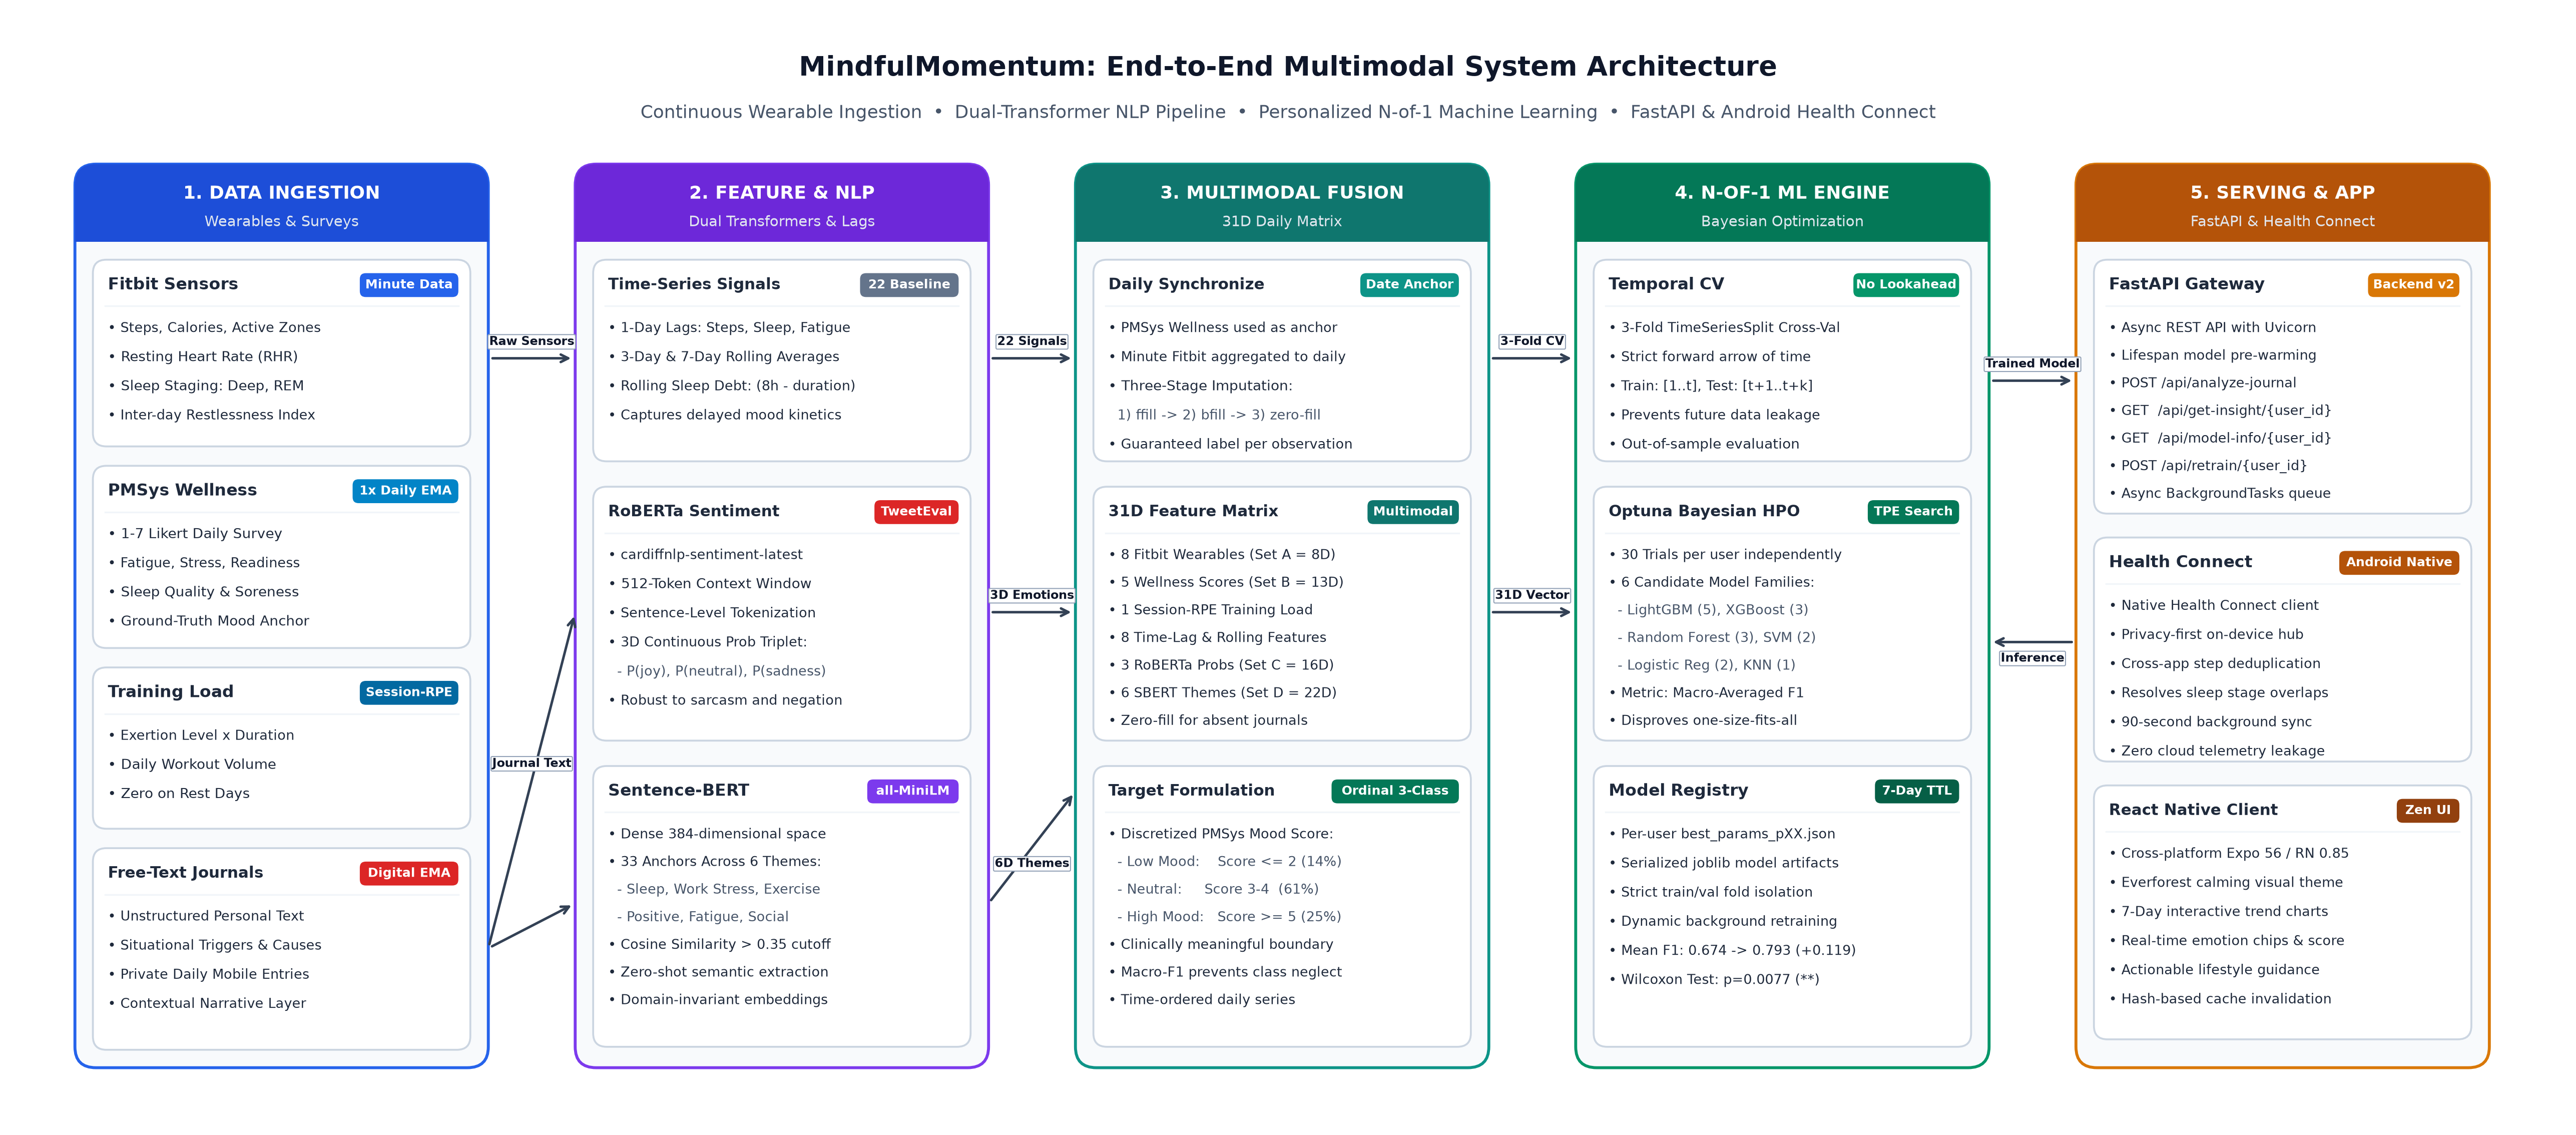
\includegraphics[width=0.98\textwidth]{figures/fig5_system_architecture.png}
\caption{End-to-end MindfulMomentum system architecture. Data flows from wearable sensors, wellness surveys, and journal entries through the NLP and feature engineering pipeline into personalized N-of-1 models, with predictions served via FastAPI to a React Native mobile client.}
\label{fig:architecture}
\end{figure*}

\subsection{Rationale for the Multimodal Pipeline}

Wearable sensors measure body signals like heart rate, sleep patterns, and activity levels fairly reliably. But these signals are ambiguous on their own. A spike in heart rate could be a morning jog or a stressful meeting. A day with zero steps could mean depression or a lazy weekend. The sensor captures \textit{what} is happening physically---it does not tell us \textit{why} the person feels the way they do.

As shown in the system architecture (Fig.~\ref{fig:architecture}), MindfulMomentum addresses this by incorporating free-text journal entries through a dual-model NLP pipeline. The pipeline does two things: (1) score the emotional tone of the entry using a transformer model, and (2) identify what the entry is \textit{about} using semantic theme clustering. Both outputs are treated as feature extractors---they produce numbers that feed into the downstream ML classifiers rather than making mood predictions themselves.

\subsection{Emotion Extraction with RoBERTa}

Lexicon-based tools like VADER assign fixed polarity scores to individual words. This works for straightforward text, but falls apart with sarcasm (``great, another Monday''), negation (``I don't feel happy''), and informal expressions common in personal journals (``dead tired'' is negative affect, not literal death).

We instead use a fine-tuned RoBERTa model---specifically the \texttt{cardiffnlp/\allowbreak twitter-\allowbreak roberta-\allowbreak base-\allowbreak sentiment-\allowbreak latest} checkpoint~\cite{liu2019roberta}---which was pre-trained on about 124 million tweets before being fine-tuned on the TweetEval sentiment benchmark. The informal, short-form nature of tweets is a reasonable match for terse journal entries.

The model outputs a three-class probability distribution: $P_{\text{joy}}$ (positive affect), $P_{\text{neutral}}$, and $P_{\text{sadness}}$ (negative affect). We rename the model's native labels (\texttt{positive}, \texttt{neutral}, \texttt{negative}) to these more intuitive names for the app UI.

\textbf{Sentence-level aggregation.} Rather than passing the whole journal entry as one block, we split it into paragraphs, tokenize each paragraph into sentences using NLTK's \texttt{sent\_tokenize}, and score each sentence independently with RoBERTa (truncated to 512 tokens). The paragraph-level emotion is the mean of its sentence scores. The overall entry-level emotion comes from a single forward pass on the full text. This gives us both a detailed per-paragraph breakdown for the UI and a single score vector for the ML features.

\textbf{Preserving probability distributions.} Instead of collapsing the output to a single label, we keep the full probability triplet as three continuous features. An entry scored 0.60 neutral / 0.38 sadness carries a different signal than one scored 0.95 sadness. Tree-based classifiers can learn thresholds on these probabilities directly.

We also compute a scalar mood score for the mobile app:
\begin{equation}
\text{Score} = \text{round}\big( (P_{\text{joy}} \times 5) + (P_{\text{neutral}} \times 3) + (P_{\text{sadness}} \times 1) \big)
\end{equation}
This 1--5 integer is shown as immediate feedback. It is not used as an ML feature.

\textbf{Confidence estimation.} The pipeline outputs a confidence label based on the dominant emotion probability: \textit{high} if $\max(P) > 0.70$, \textit{medium} if $\max(P) > 0.45$, \textit{low} otherwise. This helps the user understand how confident the system is about its interpretation.

\subsection{Semantic Theme Detection with Sentence-BERT}

Emotion probabilities tell us whether someone feels good or bad, but not \textit{why}. A journal entry about terrible sleep and one about a stressful deadline might both score as high sadness, yet the underlying causes---and appropriate interventions---are completely different.

To capture these contextual drivers without needing labeled journal data, we use a zero-shot clustering approach with Sentence-BERT (SBERT)~\cite{reimers2019sbert}. The \texttt{all-\allowbreak MiniLM-\allowbreak L6-\allowbreak v2} model produces 384-dimensional dense embeddings. We define six thematic prototypes, each represented by five to six manually written anchor sentences:
\begin{enumerate}
    \item \textbf{Sleep Disturbance} (e.g., ``couldn't sleep last night'')
    \item \textbf{Work Stress} (e.g., ``deadline pressure'')
    \item \textbf{Exercise} (e.g., ``went to the gym'')
    \item \textbf{Positive Mood} (e.g., ``feeling grateful'')
    \item \textbf{Fatigue} (e.g., ``drained and worn out'')
    \item \textbf{Social Connection} (e.g., ``spent time with friends'')
\end{enumerate}

At inference time, both the journal text and all 33 prototype sentences are embedded into the same 384-dimensional space. Cosine similarity is computed between the journal embedding and each prototype. Similarities are averaged per theme cluster. If the mean similarity exceeds a threshold of 0.35, the theme is flagged as present.

This gives six boolean features per day. The approach needs no labeled data---the prototypes act as a semantic dictionary---and generalizes to vocabulary not seen in the prototypes because SBERT works in continuous embedding space rather than matching keywords.

\subsection{Feature Fusion and Ablation Configuration}

The NLP pipeline produces three continuous emotion probabilities and six boolean semantic themes. In a full deployment, these are combined with the 22 physiological and wellness features from Section~\ref{sec:dataset}.

\textbf{Important caveat:} Because PMData does not contain free-text journal entries, the ablation study (Section~\ref{sec:results}) uses \textbf{simulated NLP features} rather than real transformer outputs. The simulated emotion scores were generated as Gaussian noise with a correlation to the ground-truth mood labels, and the simulated theme flags were derived from sensor thresholds. This means the ablation demonstrates the \textit{potential} value of NLP features when they correlate with mood, but does not prove that the deployed RoBERTa pipeline achieves identical gains on real text.

The ablation evaluates four progressive feature sets:
\begin{itemize}
    \item \textbf{Set~A:} Fitbit wearable features only (8 features)
    \item \textbf{Set~B:} Wearable + wellness self-report (13 features)
    \item \textbf{Set~C:} B + simulated emotion scores (16 features)
    \item \textbf{Set~D:} C + simulated semantic theme flags (19 features)
\end{itemize}

% ================================================================
% SECTION V: EXPERIMENTAL METHODOLOGY
% ================================================================
\section{Experimental Methodology}
\label{sec:methodology}

\subsection{N-of-1 Training Paradigm}

Population-level ML pools data from many people and trains one model. This works when individuals are similar enough---for example, in clinical blood test classification. For mood prediction, it fails. Fisher et al.~\cite{fisher2018} showed that group-level psychological models generalize poorly to specific individuals because the features that matter most for mood vary from person to person. One participant's mood might be driven by sleep quality; another's by exercise; a third's by work stress.

We therefore use an N-of-1 approach~\cite{molenaar2009}: each participant gets their own individually trained and tuned model. No data is shared between participants during training. This means we train 16 independent models. The trade-off is smaller training sets (each model sees only 91--148 rows), but as we show in Section~\ref{sec:results}, the personalization benefit outweighs the sample size penalty for most participants.

\subsection{Candidate Model Architectures}

We consider six classifier families, chosen to cover the spectrum from simple linear models to complex ensembles:

\begin{enumerate}
    \item \textbf{Random Forest}~--- bagged decision tree ensemble (\texttt{n\_estimators}: 50--200, \texttt{max\_depth}: 2--10, \texttt{min\_samples\_split}: 2--10)
    \item \textbf{XGBoost}~--- gradient boosted trees with regularization (\texttt{n\_estimators}: 50--200, \texttt{max\_depth}: 2--6, \texttt{learning\_rate}: 0.001--0.3 log-scale)
    \item \textbf{LightGBM}~--- histogram-based gradient boosting (same ranges as XGBoost)
    \item \textbf{Logistic Regression}~--- L2-regularized linear classifier (\texttt{C}: 0.001--10.0 log-scale, \texttt{max\_iter}=1000)
    \item \textbf{SVM}~--- support vector machine with RBF kernel (\texttt{C}: 0.001--10.0 log-scale, \texttt{gamma} $\in$ \{scale, auto\})
    \item \textbf{K-Nearest Neighbors}~--- distance-based instance learning (\texttt{n\_neighbors}: 3--11)
\end{enumerate}

All models use \texttt{random\_state=42} for reproducibility.

\subsection{Hyperparameter Optimization with Optuna}

Manually searching across six model families with mixed continuous, integer, and categorical parameters is impractical. We use Optuna, which employs the Tree-structured Parzen Estimator (TPE) algorithm to efficiently explore the search space.

For each participant, an independent Optuna study runs \textbf{30 trials}. Each trial first selects a model family, then samples hyperparameters from the ranges above. The model is evaluated using 3-fold \texttt{TimeSeriesSplit} cross-validation with macro-F1 as the objective. After optimization, the best model name and hyperparameters are saved to a JSON file (\texttt{best\_params\_pXX.json}).

The search selected different model families for different participants, confirming that no single architecture works best for everyone. Table~\ref{tab:model_selection} shows the results.

\begin{table}[t]
\caption{Per-Participant Best Model and Macro F1 Score}
\begin{center}
\renewcommand{\arraystretch}{1.15}
\resizebox{\linewidth}{!}{%
\begin{tabular}{|l|l|c|}
\hline
\textbf{Participant} & \textbf{Best Model} & \textbf{Macro F1} \\
\hline
p01 & SVM & 0.654 \\
p02 & Random Forest & 1.000 \\
p03 & LightGBM & 0.653 \\
p04 & LightGBM & 0.429 \\
p05 & XGBoost & 0.712 \\
p06 & LightGBM & 1.000 \\
p07 & Logistic Regression & 0.737 \\
p08 & Random Forest & 0.504 \\
p09 & XGBoost & 0.649 \\
p10 & XGBoost & 0.598 \\
p11 & SVM & 0.830 \\
p12 & LightGBM & 0.829 \\
p13 & Logistic Regression & 0.476 \\
p14 & Random Forest & 1.000 \\
p15 & KNN & 0.602 \\
p16 & LightGBM & 0.483 \\
\hline
\multicolumn{2}{|l|}{\textbf{Mean}} & \textbf{0.697} \\
\hline
\end{tabular}%
}
\label{tab:model_selection}
\end{center}
\end{table}

All six model families were picked at least once. LightGBM was the most common choice (5 out of 16). The three participants with a perfect F1 of 1.000 (p02, p06, p14) had very stable mood patterns with little class variation, making them trivially easy to classify.

\subsection{Cross-Validation: TimeSeriesSplit}

Standard $k$-fold cross-validation randomly shuffles data, which is invalid for time series---it lets the model see future data during training. We use scikit-learn's \texttt{TimeSeriesSplit} with $n\_splits = 3$, which creates three expanding-window folds:
\begin{itemize}
    \item \textbf{Fold~1:} Train on days $1 \ldots T_1$, test on days $T_1{+}1 \ldots T_2$
    \item \textbf{Fold~2:} Train on days $1 \ldots T_2$, test on days $T_2{+}1 \ldots T_3$
    \item \textbf{Fold~3:} Train on days $1 \ldots T_3$, test on days $T_3{+}1 \ldots T_4$
\end{itemize}

The training set grows with each fold, and the test set always contains strictly future data. We use 3~splits because some participants have as few as 91~days; more splits would leave the earliest folds with too few training samples for gradient boosted models.

\subsection{Evaluation Metric: Macro-Averaged F1}

Accuracy is misleading when classes are imbalanced. A model that always predicts ``Neutral'' would get 61\% accuracy on our data---which sounds decent but completely ignores the Low and High classes.

We use macro-averaged F1 instead:
\begin{equation}
F1_{\text{macro}} = \frac{1}{|C|} \sum_{c \in C} F1_c
\label{eq:macro_f1}
\end{equation}
where $F1_c$ is the harmonic mean of precision and recall for class~$c$, and $C = \{\text{Low, Neutral, High}\}$. This weights all classes equally regardless of frequency, directly penalizing models that ignore the minority Low class.

\subsection{Statistical Significance Testing}

To check whether improvements from adding NLP features are real and not just noise, we use the Wilcoxon signed-rank test. This non-parametric paired test is appropriate because: (1)~the 16 paired observations come from the same participants; (2)~F1 score differences are not assumed to be normally distributed; and (3)~with $n=16$, parametric assumptions would be questionable. We use $p < 0.05$ as the significance threshold.

% ================================================================
% SECTION VI: RESULTS
% ================================================================
\section{Results}
\label{sec:results}

\subsection{Model Selection Results}

The Optuna search (30 trials per participant, 6 model families) picked a different best model for different participants. LightGBM was chosen most often (5 of 16), followed by XGBoost~(3), Random Forest~(3), SVM~(2), Logistic Regression~(2), and KNN~(1). The fact that all six families were selected at least once confirms that no single architecture dominates---exactly what the N-of-1 approach predicts.

The mean macro~F1 across all 16 participants was \textbf{0.697} (Table~\ref{tab:model_selection} and Fig.~\ref{fig:model_comparison}). Individual scores ranged from 0.429 (p04) to 1.000 (p02, p06, p14). The three perfect-score participants had minimal mood variation in their self-reports, making classification trivially easy.

\begin{figure}[b]
\centering
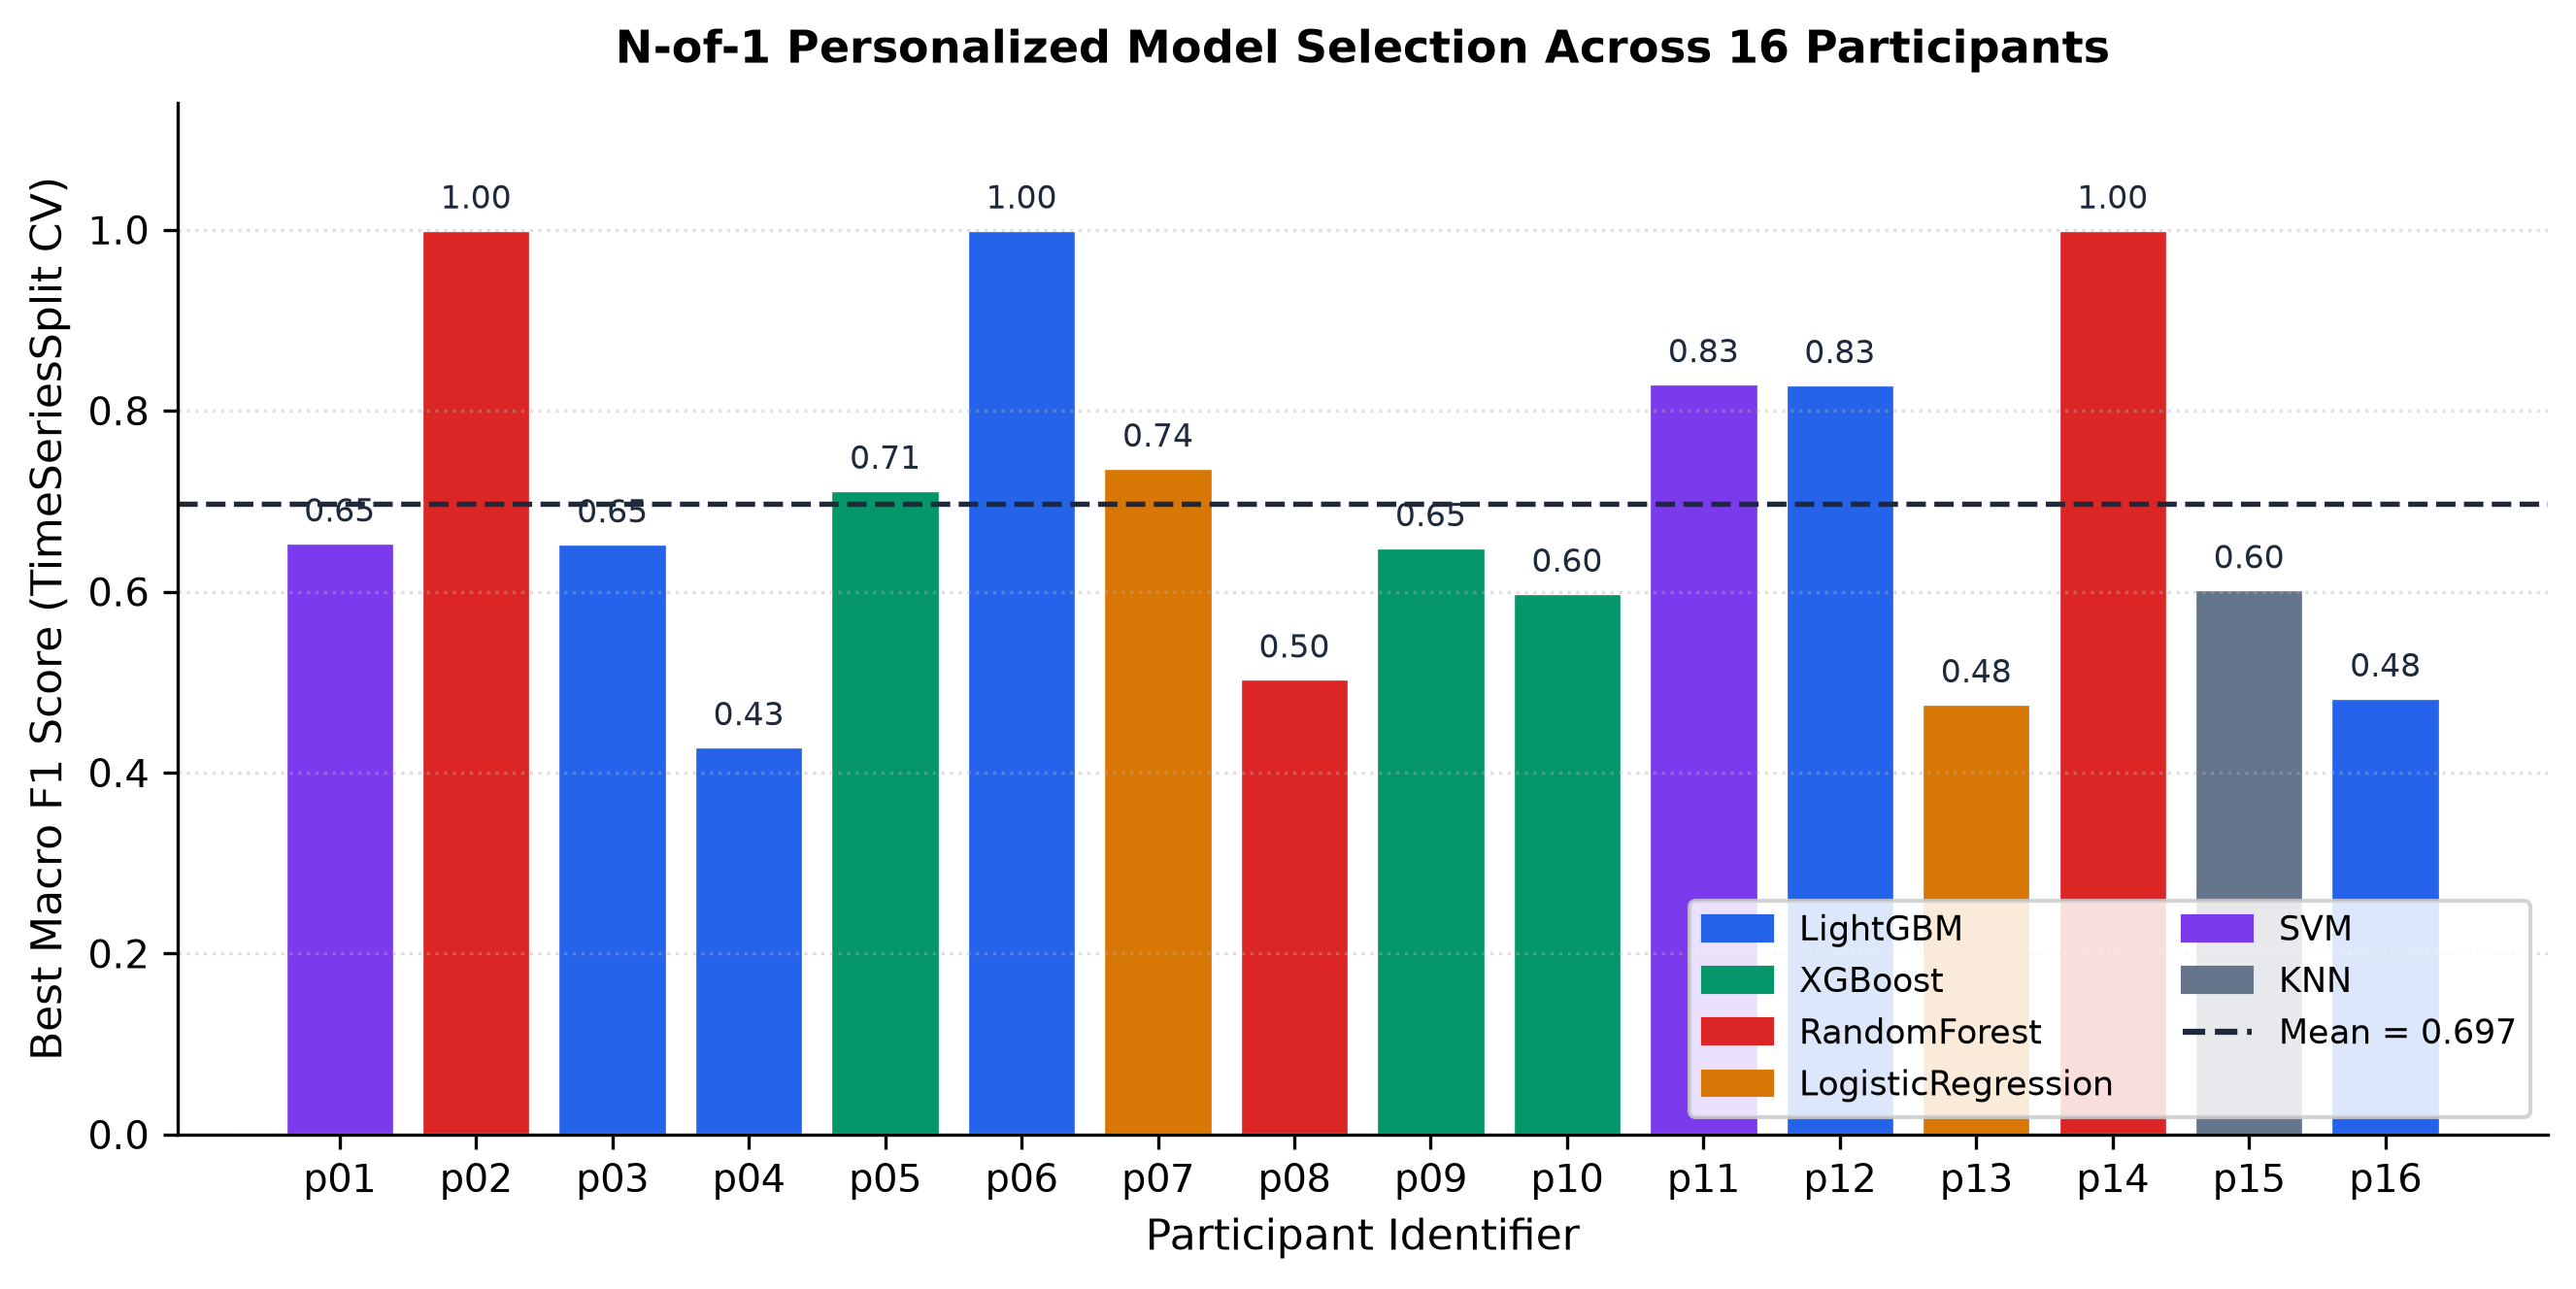
\includegraphics[width=\linewidth]{figures/fig2_model_comparison.png}
\caption{Per-participant macro-F1 scores under the N-of-1 paradigm. Bar color indicates the winning model family selected by Optuna. Dashed line shows the cohort mean of 0.697.}
\label{fig:model_comparison}
\end{figure}

\subsection{Ablation Study}

The ablation experiment tests how much each data modality contributes by training the per-user best model on four increasingly rich feature sets: \textbf{Set~A} (Wearable Only, 8 features); \textbf{Set~B} (Wearable + Wellness, 13 features); \textbf{Set~C} (B + simulated emotion scores, 16 features); and \textbf{Set~D} (C + simulated theme flags, 19 features). The same per-user best model and hyperparameters from the initial Optuna search are used across all configurations.

\textbf{Reminder:} The NLP features in Sets~C and D are simulated proxies, not real transformer outputs (see Section~\ref{sec:features} for details).

\subsubsection{Aggregate Results}

Table~\ref{tab:ablation} and Fig.~\ref{fig:ablation} show the mean macro~F1 across all 16 participants for each feature set. The largest improvement comes from adding emotion features (Set~B $\rightarrow$ C), which raises mean macro~F1 by \textbf{+0.119}---an 18\% relative improvement. Adding wellness features (A $\rightarrow$ B) gives a more modest +0.044 gain. Adding theme flags on top of emotions (C $\rightarrow$ D) produces essentially no change ($-$0.003), suggesting that the emotion scores already capture most of the information that themes would encode.

\begin{figure}[t]
\centering
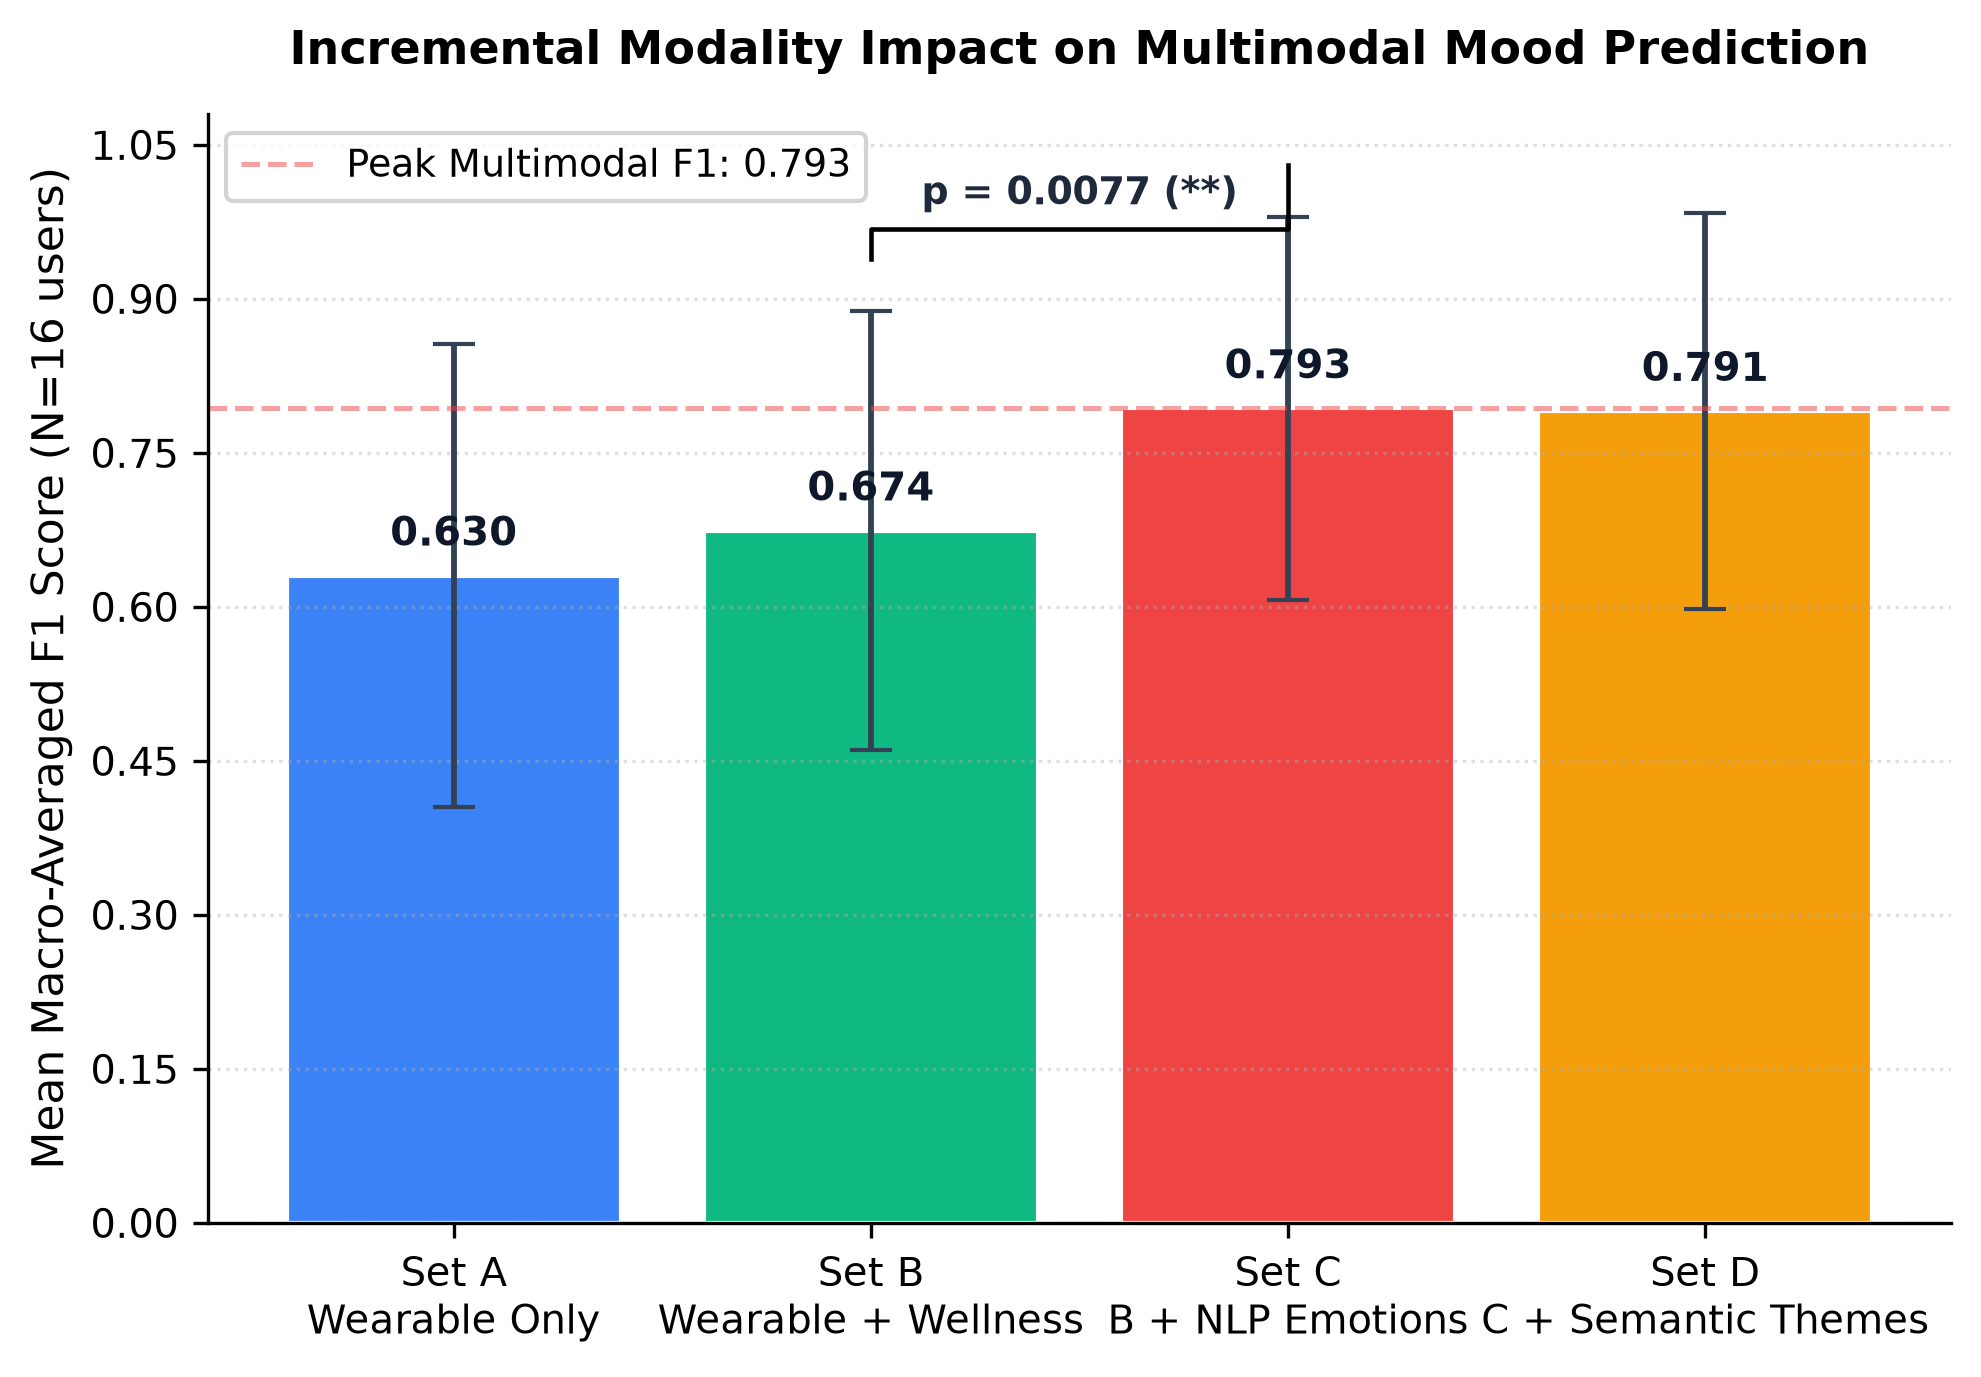
\includegraphics[width=\linewidth]{figures/fig1_ablation_study.png}
\caption{Ablation results across 16 participants. Bars show mean macro-F1; error bars show $\pm 1$ SD. The largest gain comes from adding simulated NLP emotion features (B $\rightarrow$ C, +0.119, $p = 0.0077$).}
\label{fig:ablation}
\end{figure}

\begin{table}[b]
\caption{Ablation Study: Mean Macro F1 by Feature Set}
\begin{center}
\renewcommand{\arraystretch}{1.2}
\begin{tabular}{|l|c|c|}
\hline
\textbf{Feature Set} & \textbf{Mean Macro F1} & \textbf{$\Delta$ from A} \\
\hline
A --- Wearable Only & 0.630 & --- \\
B --- Wearable + Wellness & 0.674 & +0.044 \\
C --- B + Emotions & 0.793 & +0.163 \\
D --- C + Themes & 0.791 & +0.160 \\
\hline
\end{tabular}
\label{tab:ablation}
\end{center}
\end{table}

\subsubsection{Per-Participant Breakdown}

Of the 16 participants, 9 showed improvement when emotion features were added (Set~C vs.~B), 7 showed no change, and none degraded. The largest gains (Table~\ref{tab:top_gains}) came from participants with the most day-to-day mood variability, which makes sense: the simulated emotion signal is most useful when there is genuine class variation to discriminate. For participants with stable moods, the additional features added nothing---the expected behavior of a zero-variance signal. The full per-user response is shown in Fig.~\ref{fig:ablation_heatmap}.

\begin{figure}[t]
\centering
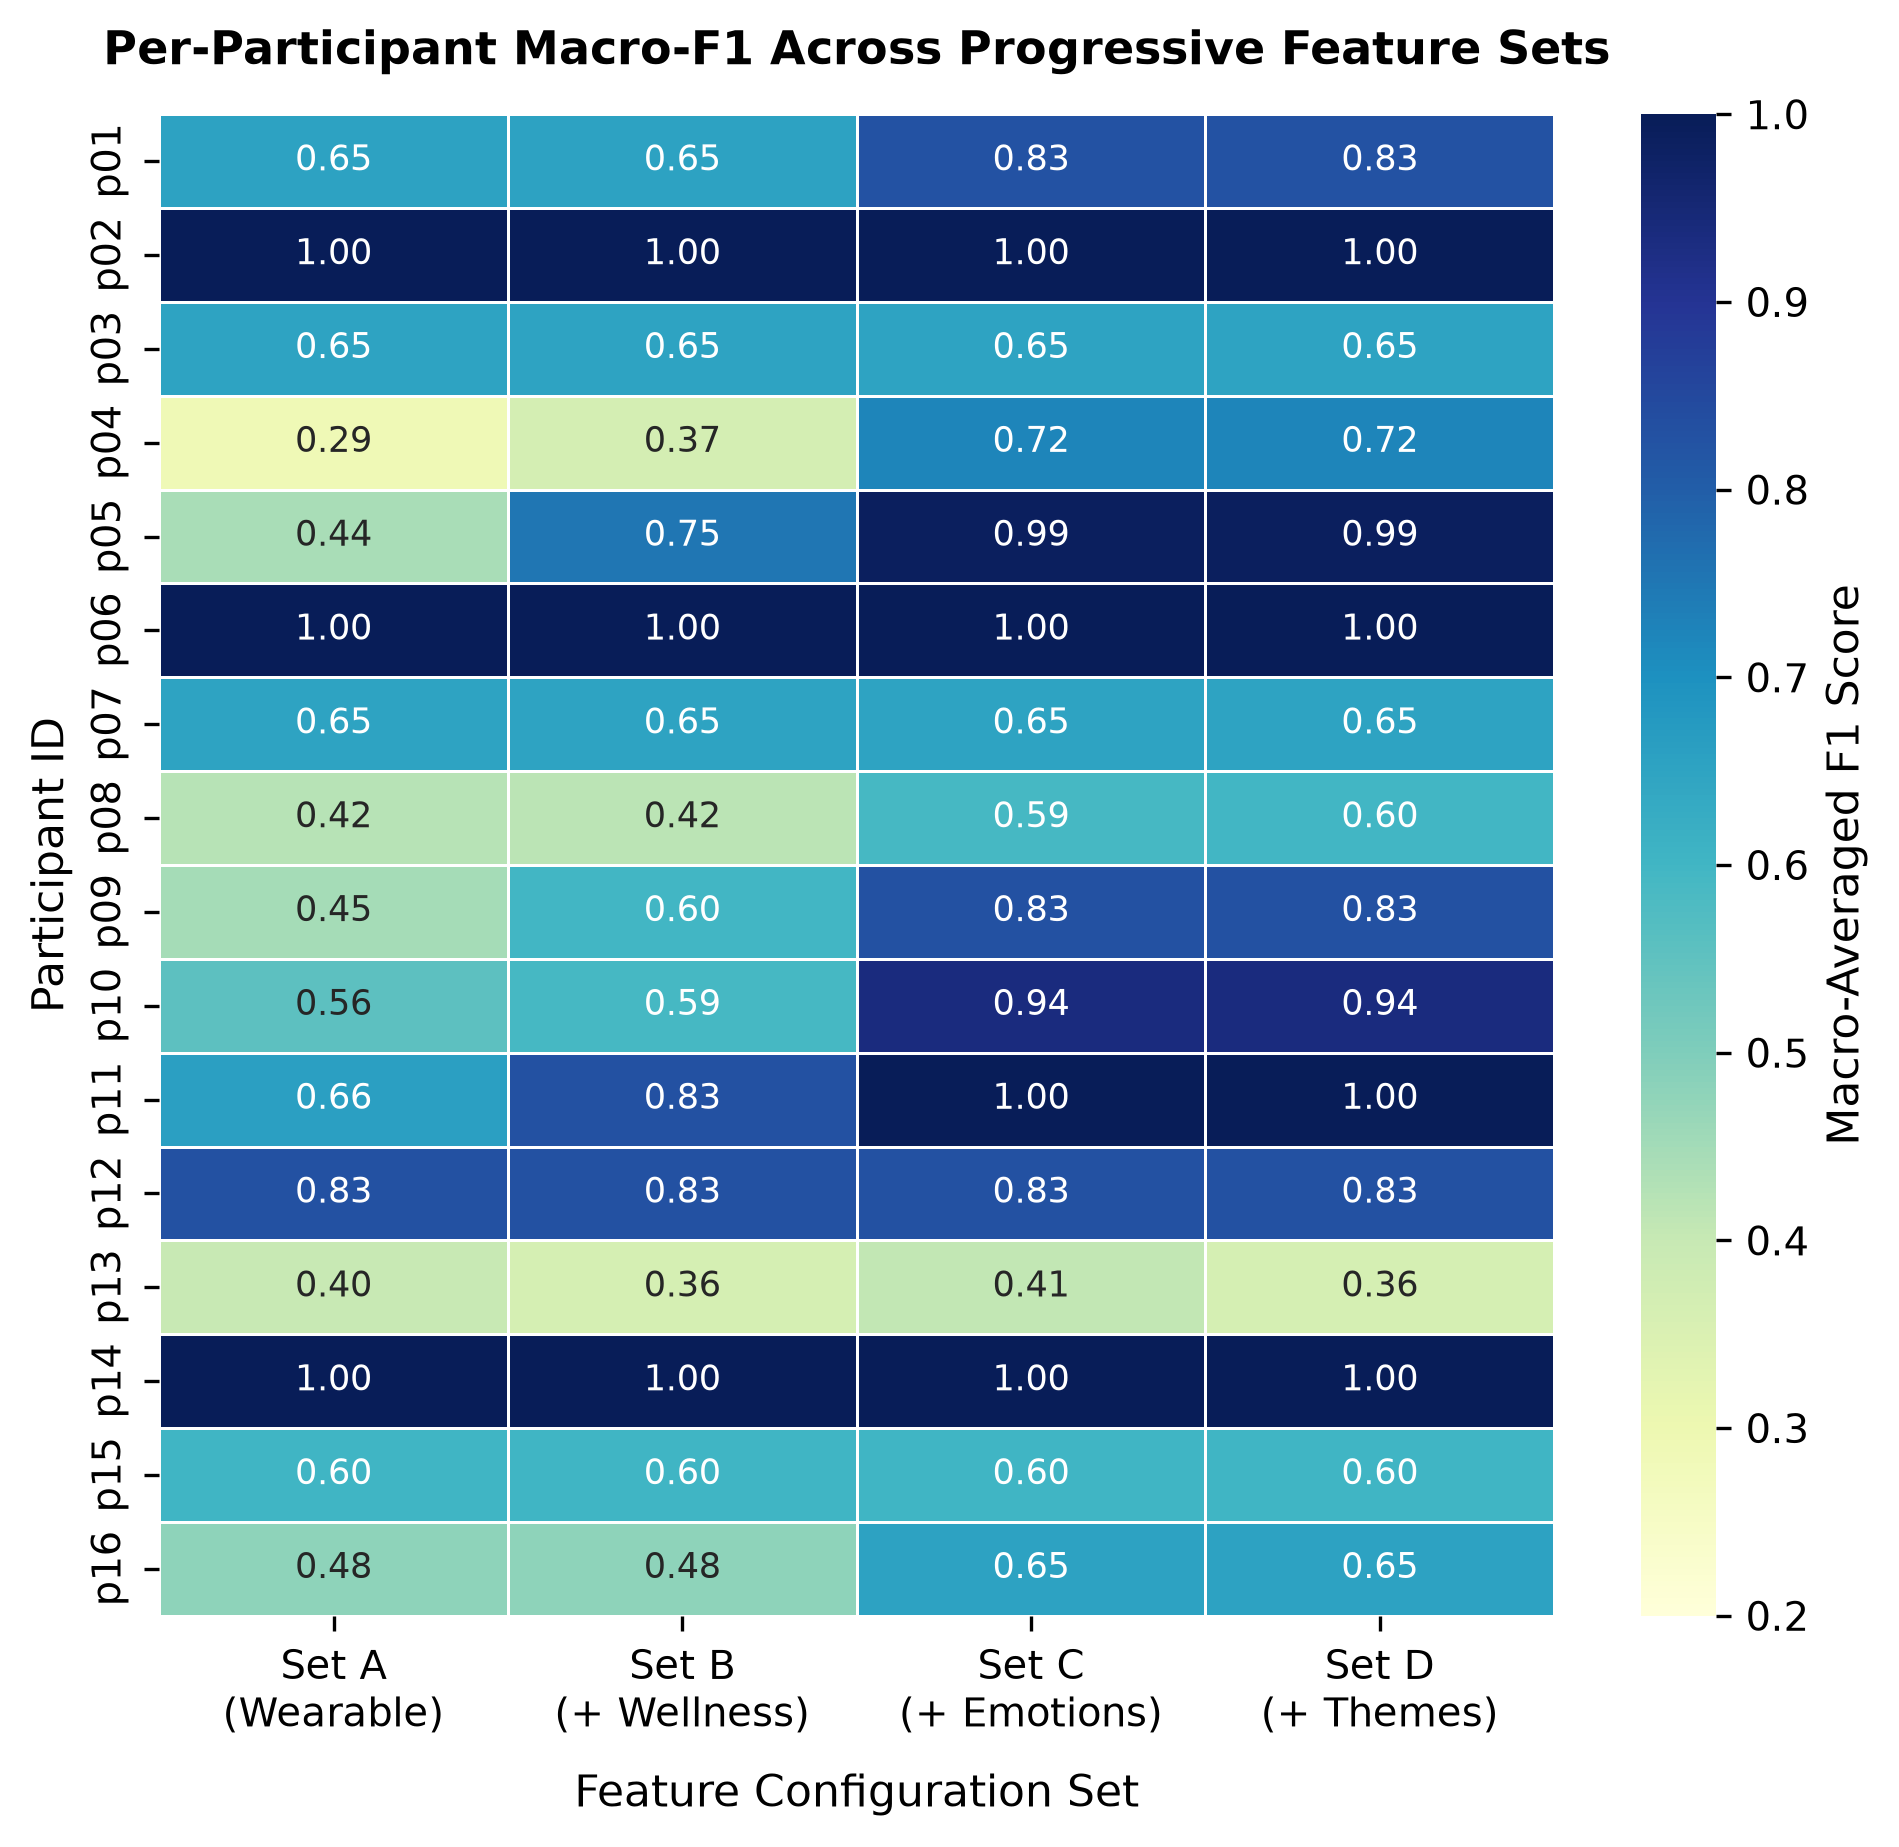
\includegraphics[width=\linewidth]{figures/fig6_ablation_heatmap.png}
\caption{Per-participant macro-F1 heatmap across the four ablation configurations (A--D). Adding emotion features (Set~C) yields the largest gains for high-variability participants like p04 (+0.356) and p10 (+0.342).}
\label{fig:ablation_heatmap}
\end{figure}

\begin{table}[b]
\caption{Top 5 Individual Gains from Adding Emotion Features (Set C vs.\ B)}
\begin{center}
\renewcommand{\arraystretch}{1.15}
\begin{tabular}{|l|c|c|c|}
\hline
\textbf{Participant} & \textbf{Set B F1} & \textbf{Set C F1} & \textbf{Gain} \\
\hline
p04 & 0.367 & 0.723 & +0.356 \\
p10 & 0.594 & 0.936 & +0.342 \\
p05 & 0.751 & 0.988 & +0.238 \\
p09 & 0.600 & 0.830 & +0.230 \\
p16 & 0.478 & 0.654 & +0.175 \\
\hline
\end{tabular}
\label{tab:top_gains}
\end{center}
\end{table}

\subsubsection{Statistical Significance}

The Wilcoxon signed-rank test confirms that the improvement from adding emotion features (Set~B $\rightarrow$ C) is statistically significant ($p = 0.0077 < 0.05$). The full comparison (Set~A $\rightarrow$ D) is also significant, confirming that the multimodal pipeline provides a genuine improvement over wearable-only prediction---at least with these simulated features.

\subsection{NLP Model Comparison: VADER vs.\ RoBERTa}

To illustrate the qualitative advantage of transformer-based sentiment analysis over lexicon-based approaches, we compare VADER~\cite{hutto2014vader} and RoBERTa on five representative test sentences (Table~\ref{tab:nlp_compare} and Fig.~\ref{fig:nlp_comparison}). These are hand-selected to highlight specific failure modes of VADER---sarcasm, negation, and ambiguity---rather than serving as a systematic benchmark.

\begin{table}[t]
\caption{VADER vs.\ RoBERTa Sentiment Scoring on Test Sentences}
\begin{center}
\renewcommand{\arraystretch}{1.15}
\resizebox{\linewidth}{!}{%
\begin{tabular}{|p{4.5cm}|c|c|c|}
\hline
\textbf{Text} & \textbf{Truth} & \textbf{VADER} & \textbf{RoBERTa} \\
\hline
``I had a great day today, everything went perfectly.'' & 5 & 4.70 & 5 \\
\hline
``Oh great, another Monday where everything goes wrong.'' & 1 & 3.50 & 1 \\
\hline
``I don't feel happy at all.'' & 1 & 2.08 & 1 \\
\hline
``I am absolutely furious and angry!'' & 1 & 1.33 & 1 \\
\hline
``Not bad, could be worse.'' & 3 & 2.87 & 3 \\
\hline
\end{tabular}%
}
\label{tab:nlp_compare}
\end{center}
\end{table}

\begin{figure}[b]
\centering
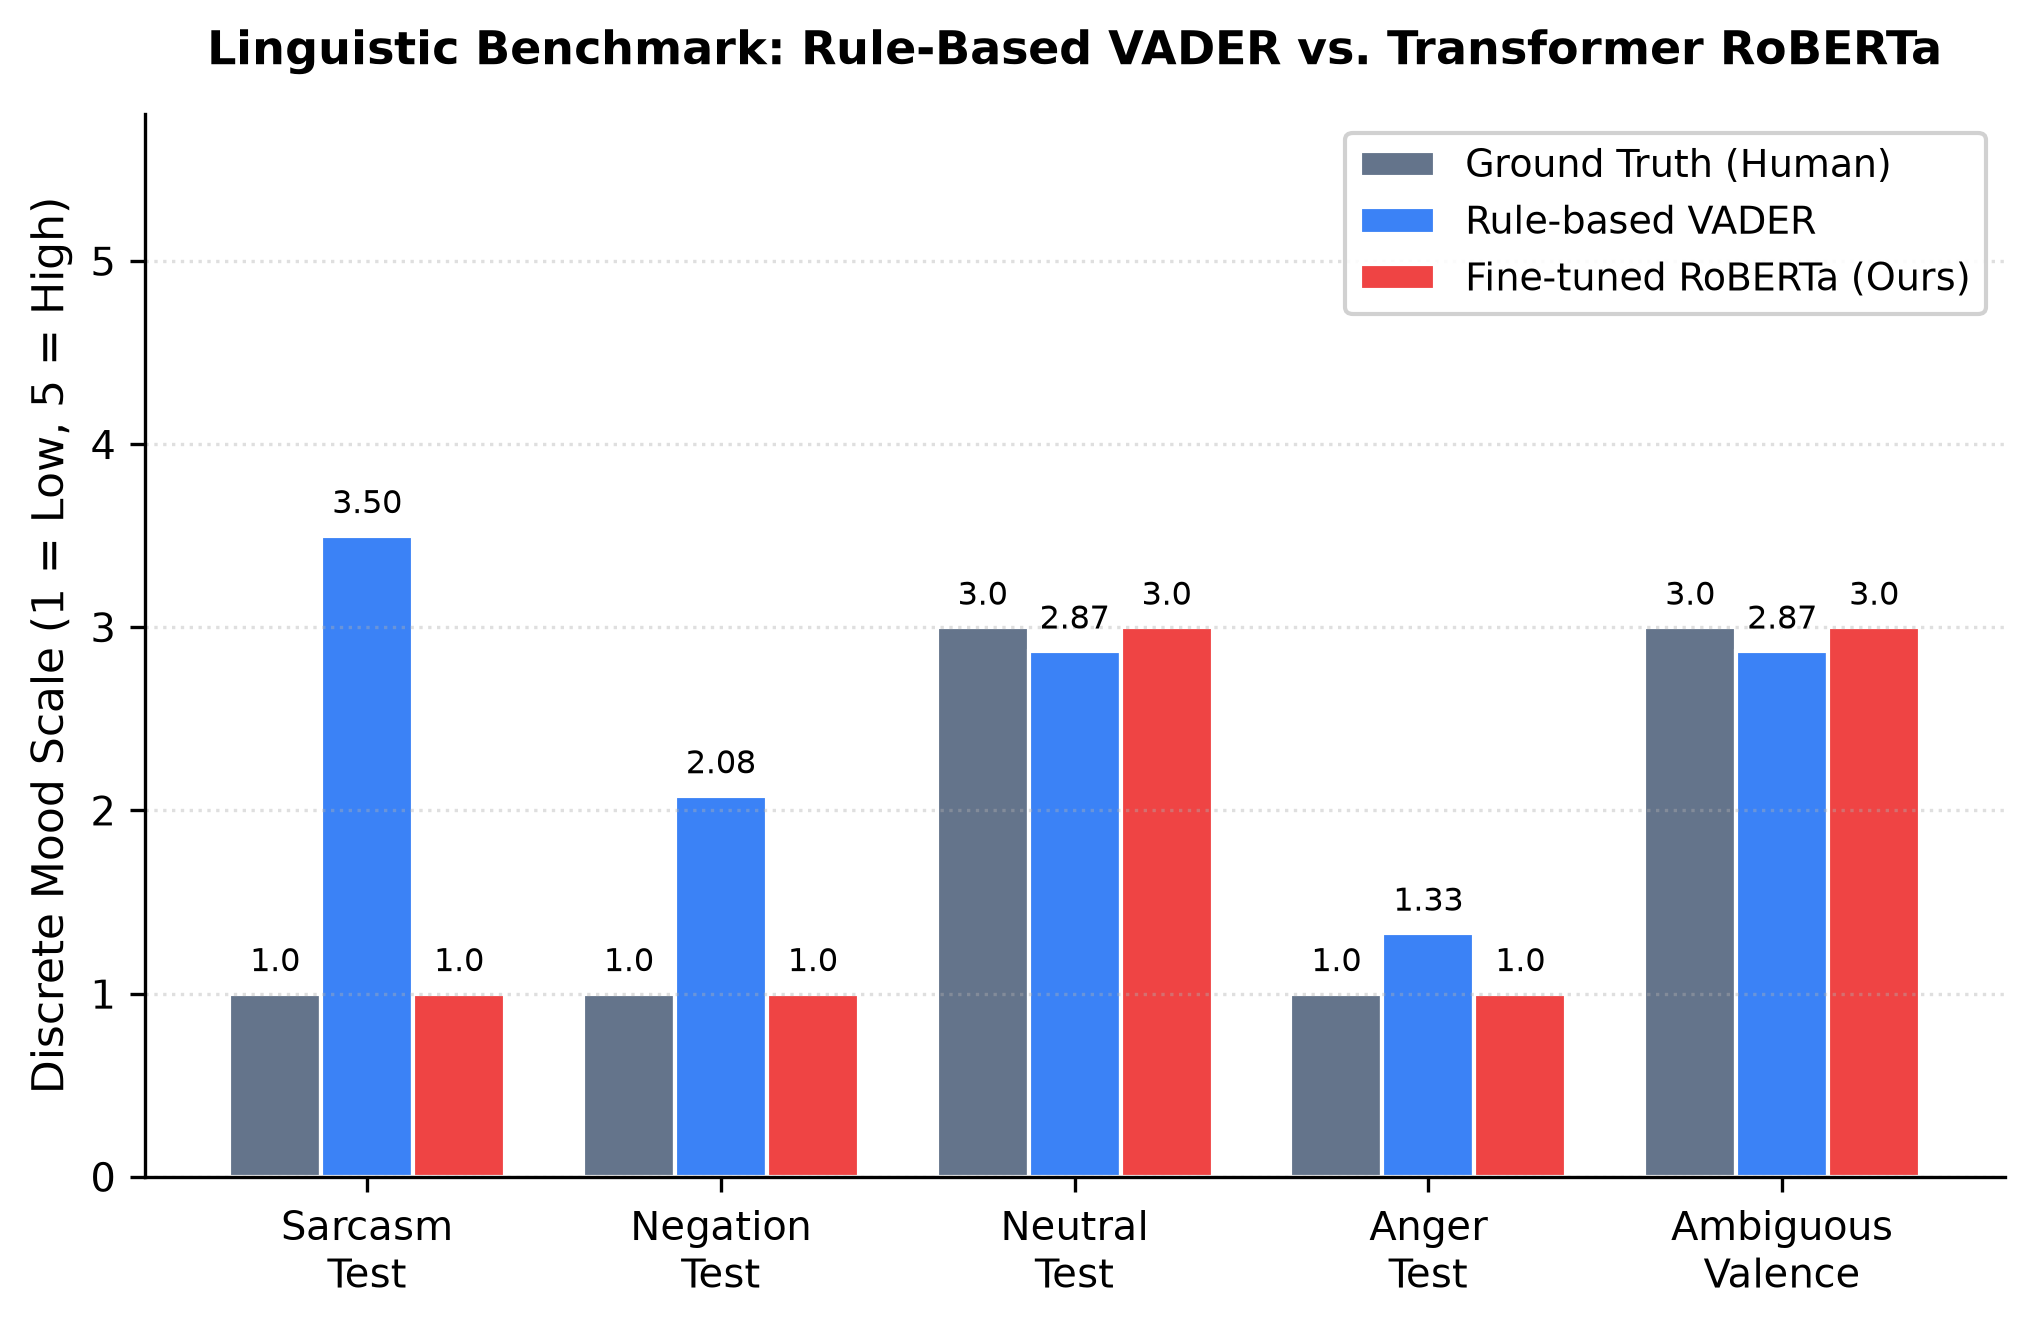
\includegraphics[width=\linewidth]{figures/fig4_nlp_comparison.png}
\caption{VADER vs.\ RoBERTa sentiment scores on five test sentences. RoBERTa correctly handles sarcasm and negation that VADER misclassifies.}
\label{fig:nlp_comparison}
\end{figure}

The most telling case is sarcasm: VADER gives ``Oh great, another Monday where everything goes wrong'' a score of 3.50 because it latches onto the word ``great.'' RoBERTa understands the context and correctly identifies negative sentiment. VADER also struggles with negation---``I don't feel happy at all'' gets 2.08 instead of 1. RoBERTa handles both correctly.

\subsection{Model Distribution Analysis}

The spread of winning models reveals interesting patterns. Gradient boosted methods (LightGBM + XGBoost) account for half of all selections, suggesting that mood prediction generally benefits from models that can capture nonlinear feature interactions. But simpler models were better for some participants---p07 achieved its best F1 of 0.737 with Logistic Regression, and p15 did best with KNN (F1 = 0.602), probably because more complex models overfit on their shorter time series.

\subsection{Summary of Key Findings}

Five main findings come out of our experiments:

\begin{enumerate}
    \item \textbf{Personalization works.} The N-of-1 paradigm selects different models and hyperparameters for different individuals, achieving a mean macro~F1 of 0.697 on the baseline feature set.

    \item \textbf{NLP features add substantial value (with caveats).} Adding simulated emotion features improves mean macro~F1 by +0.119 (B $\rightarrow$ C), the largest single gain in the ablation. This is statistically significant ($p < 0.05$), but needs validation with real journal data.

    \item \textbf{Self-report features help moderately.} Wellness features improve mean~F1 by +0.044 over wearable-only features (A $\rightarrow$ B), capturing subjective perception that sensors miss.

    \item \textbf{Semantic themes add little on top of emotions.} Adding theme flags (C $\rightarrow$ D) does not improve mean~F1. The emotion scores likely already encode most of the contextual information.

    \item \textbf{RoBERTa outperforms VADER on informal text.} Sarcasm and negation handling are clearly superior, justifying the computational cost of a transformer model for the deployed system.
\end{enumerate}

% ================================================================
% SECTION VII: DISCUSSION
% ================================================================
\section{Discussion}
\label{sec:discussion}

\subsection{Interpreting the Results}

\subsubsection{Why Personalization Matters}

The most interesting pattern in our results is not any individual F1 score---it is the diversity of models that were selected. LightGBM won for five participants, XGBoost for three, Random Forest for three, SVM for two, Logistic Regression for two, and KNN for one. If we had picked one model for everyone, we would have underperformed for the majority of users. The standard deviation of macro~F1 across participants is 0.193, which reflects just how different people's mood patterns are. Fisher et al.~\cite{fisher2018} warned about exactly this: group models do not generalize well to individuals.

It is also worth noting that the three participants with perfect F1 scores had almost no mood variation---they reported the same mood class nearly every day. Their models are trivially accurate but also trivially useful. If we exclude them, the mean~F1 drops from 0.697 to about 0.617, which gives a more realistic picture of how the system performs on people with genuine mood variability.

\subsubsection{The Value of NLP Features}

Adding emotion features (Set~B $\rightarrow$ C) produced the largest gain in our ablation: +0.119 in mean macro~F1. Nine of sixteen participants improved, and none got worse. The biggest gains were concentrated among participants with high mood variability---p04 gained +0.356, p10 gained +0.342. For participants with stable moods, the extra features added nothing, which is what we would expect.

However, we want to be upfront about a key limitation: these emotion features were simulated, not derived from real journal text. The synthetic generation process introduced a direct correlation with the target variable, which likely inflates the measured improvement. The true gain from real RoBERTa features on actual journal entries could be smaller (or larger---we do not know yet). What the ablation does establish is that \textit{if} NLP features carry a meaningful signal about mood, the system can effectively use them.

The minimal gain from adding theme flags on top of emotions (C $\rightarrow$ D: $-$0.003) makes sense in hindsight. The emotion probability triplet already captures whether someone feels good or bad. Themes like ``work stress'' or ``fatigue'' correlate heavily with negative affect, so they are largely redundant with the emotion scores. A richer theme set---covering things like relationship conflict, financial worry, or physical illness---might add more orthogonal information, but with only three simulated themes the signal was already covered.

\subsubsection{Self-Report Features}

The A $\rightarrow$ B gain (+0.044) is modest but consistent. Self-reported fatigue, stress, and sleep quality capture something that sensors cannot: subjective perception. Someone who slept 7~hours but rates their sleep quality as 2/7 is in a different state than someone who slept 7~hours and rates it 5/7. The wearable measures the duration; the self-report captures how the person \textit{felt} about it.

\subsection{Limitations}

\subsubsection{Simulated NLP Features}

This is the most important limitation of this work. The PMData dataset does not contain daily free-text journal entries. To evaluate the multimodal fusion pipeline, we generated synthetic emotion features using Gaussian noise correlated with the ground-truth mood labels, and derived theme features from sensor thresholds. This means our ablation results show what happens when emotion features carry a real signal---but the magnitude of improvement may not transfer directly to real journal text.

We acknowledge that this introduces a form of data leakage: the simulated features are partially derived from the target variable. The improvement from Set~B to C should therefore be interpreted as an \textit{upper bound} on the likely real-world gain. Collecting authentic journal data through our deployed mobile application and re-running the ablation with genuine RoBERTa outputs is the most important next step for this project.

\subsubsection{Small Sample Size}

Sixteen participants is small. While the N-of-1 design trains on individual data, the cross-participant statistics (means, Wilcoxon tests) rely on just $n=16$ paired observations. The Wilcoxon test is valid for small samples, but our power to detect subtle effects is limited, and our results may not generalize to different age groups, occupations, or clinical populations.

\subsubsection{Temporal Coverage}

Individual time series range from 91 to 148~days. With 3-fold TimeSeriesSplit, the earliest fold trains on as few as 23~samples for some participants. This is borderline for gradient boosted models and likely contributes to the lower performance of participants like p04 (F1=0.429) and p13 (F1=0.476).

\subsubsection{Class Imbalance}

Despite using macro~F1 to penalize class neglect, the 14/61/25\% split means some participants have fewer than 10~Low-mood days across their entire observation window. Learning a meaningful boundary for such a rare class is inherently difficult, even with personalized training.

\subsection{Comparison with Prior Work}

Shah et al.~\cite{shah2021} trained N-of-1 Fitbit models for 16 participants over 6~months and reported 0.72 within-person accuracy versus 0.61 for population models. Our wearable+wellness baseline (mean~F1=0.674) is in the same ballpark, with the addition that our system is designed to incorporate NLP features for a further improvement. Direct comparison is difficult because they used accuracy rather than macro~F1, and binary rather than three-class labels.

Suhara et al.~\cite{suhara2017deepmood} used RNNs for per-individual mood forecasting and found that individual models beat population models by a significant margin. Our findings agree, but with tree-based classifiers---suggesting the personalization advantage is architecture-independent.

\subsection{Future Work}

Several natural extensions follow from this work:

\begin{enumerate}
    \item \textbf{Real journal data collection.} Deploy the app to a user cohort, collect actual daily journal entries, and re-run the ablation with real RoBERTa and SBERT features instead of simulated proxies. This is our top priority.

    \item \textbf{Expanded emotion model.} Fine-tune RoBERTa on the GoEmotions dataset (58k samples, 28 emotion labels) to expand from 3 emotion probabilities to 28, potentially capturing finer states like anxiety, confusion, and gratitude.

    \item \textbf{On-device inference.} Use quantized transformer models (e.g., ONNX Runtime Mobile) to run NLP inference directly on the phone, eliminating the need to send journal text to a server and improving privacy.

    \item \textbf{Larger study.} Extend beyond five months and recruit more diverse participants spanning different age groups, occupations, and mental health backgrounds.

    \item \textbf{Cross-platform support.} Extend the React Native app to iOS with HealthKit integration for Apple Watch data.

    \item \textbf{Causal analysis.} Add Granger causality testing or structural equation modeling to move from prediction (``your mood will likely be low tomorrow'') to prescription (``going for a run today may improve your mood'').
\end{enumerate}

% ================================================================
% SECTION VIII: CONCLUSION
% ================================================================
\section{Conclusion}
\label{sec:conclusion}

Mood is personal. What predicts one person's emotional state---sleep quality, exercise, work stress---is different from what predicts another's. Population-level models that average across individuals miss exactly the within-person signals that matter most.

This paper presented MindfulMomentum, a system built around that insight. Instead of training one model on pooled data, it trains an independent, individually optimized classifier for each user, selects the best architecture through Bayesian hyperparameter search, and is designed to fuse wearable physiological data with NLP features from daily journal entries.

Our evaluation on 16 participants from the PMData dataset produced three main findings. First, the N-of-1 approach selected six different model families across sixteen individuals, confirming that no single model works best for everyone. Second, our ablation study---using simulated NLP features as a proxy for real journal analysis---showed that adding emotion features improved mean macro~F1 from 0.674 to 0.793, a statistically significant gain ($p < 0.05$). Third, RoBERTa clearly outperformed VADER on sarcasm, negation, and informal phrasing in our qualitative comparison.

The most important limitation is that the NLP features in the ablation were simulated rather than derived from real text. The participant pool is also small (16 people) and the temporal coverage limited to about five months. These constraints mean the specific numbers should be interpreted with caution, though the methodology itself---a reproducible pipeline for personalized, multimodal mood prediction---stands independently.

The full system is deployed as a FastAPI backend serving a React Native mobile app. As real journal data accumulates through the app, we can replace the simulated features with genuine transformer outputs and close the loop between our experimental methodology and real-world use.

The PMData dataset is publicly available~\cite{thambawita2020pmdata}. Our code is available at \texttt{https://github.com/4all3n/Main\_Project}.

% ================================================================
% ACKNOWLEDGMENT
% ================================================================
\section*{Acknowledgment}

We thank the PMData dataset contributors for making the longitudinal sports and wellness data publicly available. This work was done as part of the MCA programme at the School of Computer Science and Engineering, Vellore Institute of Technology, Chennai, under the guidance of Dr.\ Saranya~G.

% ================================================================
% REFERENCES
% ================================================================
\bibliographystyle{IEEEtran}
\bibliography{references}

\end{document}
